\section{Introduction}
\label{sec:introduction}

Android's open-source nature and vast app ecosystem have contributed to its widespread adoption. For regulating access to sensitive user data, Android employs a permission framework that serves as a gatekeeper~\cite{alkindi2019android}. When using an app, the Android permission framework allows the user to either grant or deny permission for each type of data individually. Unfortunately, the study by Wagner et al.~\cite{ha2013android} reveals that only 17\% of Android users pay attention to permissions while installing/using an app. Once a user grants permission to an app, the permission framework allows unrestricted access to sensitive data endangering the user's privacy~\cite{alkindi2019android}. If the user does pay attention to privacy concerns and denies a permission request, the app often blocks access to not only the features related to the permission but also other features that may not require that permission~\cite{alkindi2019android}. This leaves the user with no alternative but to provide access to their data.

\begin{figure}[t]
    \centering
    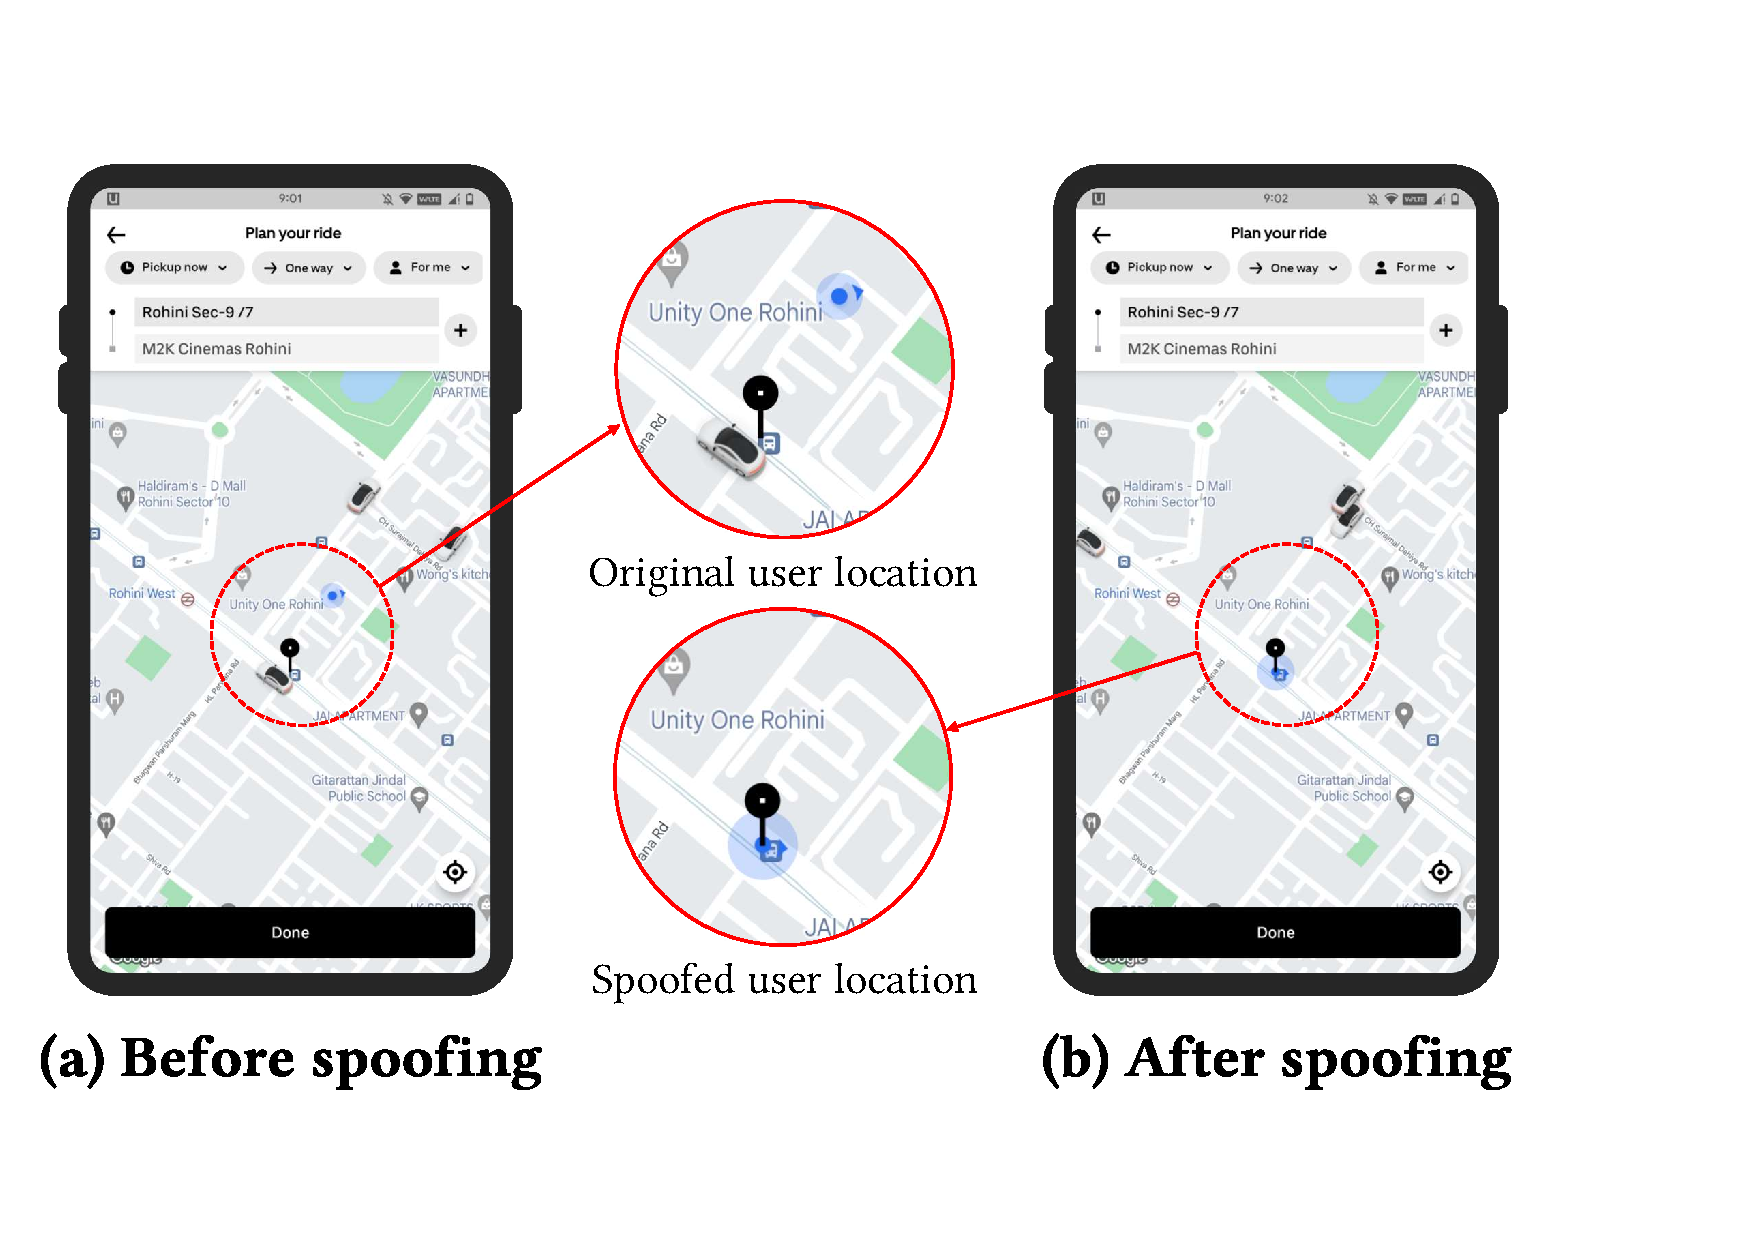
\includegraphics[width=0.75\linewidth]{Figures/Case Studies/uber_screenshots.pdf}
    \caption{Screenshots illustrating how a user can share spoofed location using \framework{} with the Uber app.}
    \label{fig:intro_case_study_uber}
    \vspace{-10pt}
\end{figure}

To enhance user privacy without limiting the app's functionality, users could be equipped with another option: feeding user-controlled, spoofed data to apps. Figure~\ref{fig:intro_case_study_uber} shows such a case study. In Figure~\ref{fig:intro_case_study_uber}a, we observe that even though the user wants to take the cab from the pinned location, Uber encourages the user to share their original location compromising their privacy. Figure~\ref{fig:intro_case_study_uber}b demonstrates how the user can hide their original location and feed the user-specified spoofed location as the current location. This safeguards the user's privacy while still enabling them to utilize Uber's service of finding a cab.

Unfortunately, existing approaches for spoofing the user data involve either modifying the Android OS~\cite{smalley2013security, raval2016you, wu2017context} or rebuilding the target app binary~\cite{backes2015boxify, jeon2012dr}, which have severe limitations in terms of usability and practicality. Modifying the OS requires rooting the device which is not practical for users~\cite{zhang2015android}. Rebuilding app binary is not always successful as it can be easily detected by using Google's Play Integrity API, making the app prevent users from accessing its services~\cite{andPlayIntAPI}. 

To equip users with a practical tool for preserving their privacy, we have built \textit{\framework{}}, a comprehensive and robust user data spoofing system that can spoof any user data fed to an app installed on a typical non-rooted Android device. Our evaluation results indicate that \framework{} robustly spoofs 78.32\% of the requested permissions by 70 popular pre-installed and user-installed Android apps without getting detected by the target apps and without crashing them.

We further show that the deception capability of \framework{} can be utilized to bypass continuous authentication mechanisms. Researchers have been developing a wide range of continuous user authentication mechanisms that rely upon device sensor data (e.g., accelerometer)~\cite{kolokas2019gait, sun2018artificial, thang2012gait, hoang2013adaptive, shih2015flick, nohara2016personal, lu2015safeguard, jain2015exploring, nixon2016slowmo, feng2014tips, abuhamad2020autosen, amini2018deepauth, li2018using, yan2018towards, song2016eyeveri, xia2018motionhacker, hong2016mgra, hong2015waving, miguel2016interaction, zhang2016voicelive, wang2019voicepop, johnson2013secure, khamis2016gazetouchpass, zhu2013sensec, sitova2015hmog, pang2019mineauth, acien2019multilock, zhu2019riskcog, lee2017implicit}. Unlike traditional one-time authentication mechanisms using passwords, a continuous authentication mechanism operates discreetly in the background, constantly monitoring user behavior and biometric features to validate their identity throughout their interaction with an app. Towards that end, to the best of our knowledge, \framework{} is the first system to demonstrate the ineffectiveness of the sensor data-based continuous authentication mechanisms in Android platforms.

\begin{table}
    {\centering
    \begin{tabular} {>{\arraybackslash\centering}m{2.5cm} >{\arraybackslash}m{9.5cm}}
        \hline
         \textbf{Use Case} & \textbf{Example(s)}\\
         \hline
         Bypassing Continuous Authentication & 
         \textbf{MGRA}~\cite{hong2016mgra} (Sec \ref{sec:continuous_authentication_mechanisms}) utilizes the accelerometer data and \textbf{VoiceLive}~\cite{zhang2016voicelive} (Sec \ref{sec:continuous_authentication_mechanisms}) utilizes the smartphone's two different microphones to authenticate users. But \framework{} proves to be capable of bypassing these authentication mechanisms by spoofing the input data. \\
         \hline
         Granting Selective User Data & 
         \textbf{Snapchat}(\hyperref[sec:sc_case_study]{Sec 5.3}) and \textbf{Truecaller}(\hyperref[sec:tc_case_study]{Sec 5.4}) requires users private data like Contacts and Messages to enable users to utilize functionalities provided by them, but this also compromises the private information. However, \framework{} enables users to grant partial data to apps that is essential.\\
         \hline
         Protection from Malicious Apps & 
         \textbf{All Good PDF Scanner} (Sec \ref{sec:malicious_apps}) was granted permissions like Storage and Camera but was detected to be uploading data on the internet in the background, hence its internet access was blocked by \framework{}. \textbf{Unique Keyboard} (Sec \ref{sec:malicious_apps}) was found to be accessing the sensor data while running in the background, therefore \framework{} fed deceived data when app is running in the background.\\
         \hline
         Side-Channel Attack Mitigation & 
         \textbf{Gyrosec}~\cite{lin2019motion} (Sec \ref{sec:side_channel_attack}) records the sensor data while running in the background, and uploads it over the internet. This was mitigated by deceiving the sensor data received by the apps.  \\
         \hline
         Unexpected Sensor Usage Detection & 
         \textbf{Facebook} (Sec \ref{sec:fb_case_study}) requested for Audio permission. But it was found (using \framework{}) to be recording the microphone data when no activity requiring microphone was being used by the user.\\
         \hline
         User Privacy Protection & 
         \textbf{Snapchat} (Sec \ref{sec:sc_case_study}) and \textbf{Truecaller} (Sec \ref{sec:tc_case_study}) provide great features to users but at the cost of sharing private information like Location, Contacts and Messages. \framework{} enables users to enjoy the provided features without compromising private information.\\
         \hline
    \end{tabular}
    }
    \caption{Various use cases of \framework{} and their respective real-world example(s)}
    \label{tab:highlights}
\end{table}

We show that \framework{} proves to be successful in detecting malicious behaviors of and protecting user's private information from malicious apps that have been recently banned by Google. For example, while experimenting with the ``All Good PDF Scanner" Android app, \framework{} detected that the app was uploading user's private files to the internet. \framework{} blocked internet access of the app without crashing or limiting features of the app.

We also demonstrate \framework{}'s potential to detect and mitigate side-channel attacks by malicious apps. For example, our experiments reveal a significant drop in the mobile screen touch position prediction capability of a side-channel attack launched by a malicious app from 81.22\% to just 5.36\% when \framework{} is employed. 

The usage of \framework{} extends beyond protection against malicious apps. We use three real-world apps as case studies to show how \framework{} gives better control over privacy to users. For example, our study of real-world apps uncovers Facebook app recording user's audio while the user is just scrolling over the posts on the home page of Facebook app. This behaviour was not informed to the user by the Android privacy indicator (green dot) but it was detected by \framework{}. \framework{} could spoof audio to protect user's privacy. 

A demonstration video of employing \framework{} for user data spoofing on the Facebook app is available on \href{https://www.youtube.com/watch?v=sXiGUoqFLmk}{Youtube}\footnote{https://www.youtube.com/watch?v=sXiGUoqFLmk}. Table \ref{tab:highlights} highlights various usages of \framework{} with examples.

We validate that spoofing sensitive user data using \framework{} introduces only a minimal average overhead of 2.52\% in battery drain and 5.2 MB of memory during app runs. Each spoofed API call adds an average of 1.64 ms of overhead which did not add any noticeable performance degradation in the apps that we tested.

Overall, we make the following key contributions.

\begin{itemize}
    % [leftmargin=*]
    \item We present \framework{}, a comprehensive and robust system that can be utilized for spoofing any user data fed into an app without rooting the device or modifying the app's source code. We show that \framework{} adds minimal overhead.
    \item The inherent design of \framework{} enables it to bypass continuous authentication mechanisms shedding light on the limitations and weaknesses present in the current implementation of these mechanisms. 
    \item We show how \framework{} mitigates direct privacy attacks and side-channel attacks by malicious apps.
    \item We demonstrate how \framework{} can protect user privacy on real-world apps such as Facebook, Snapchat, Truecaller, and Uber. 
\end{itemize}

The rest of the paper is organized as follows. Section~\ref{sec:motivation} presents the motivation for developing a system to spoof user data. Section~\ref{sec:methodology} explains the methodology employed in \framework{} to spoof user data accessed by target apps. Section~\ref{sec:architecture} presents the detailed architecture of \framework{}. Sections~\ref{sec:mitigating_sca} and \ref{sec:protecting_up} showcase usefulness of \framework{}. Section~\ref{sec:mitigating_sca} shows how \framework{} can detect and mitigate privacy attacks from malicious apps to protect user privacy. Section~\ref{sec:protecting_up} shows how \framework{} empowers users to get better control over their privacy while using bening real-world apps. Section~\ref{sec:results} provides the evaluation results on the overhead of \framework{}. Section~\ref{sec:related_work} presents an overview of prior approaches. We conclude the paper in Section~\ref{sec:conclusion}.